\documentclass[a4paper, 11pt]{article}
%\documentclass[a4paper, 10pt]{amsart}

% multi-line spacing for easier marking
%\usepackage{setspace}

% math symbols
\usepackage{amssymb,amsmath}
\usepackage{textcomp}

% nicer fonts
\usepackage{times}

% for fancy tables with multi-row headers
\usepackage{multirow}
% for pictures
\usepackage{graphicx}

\usepackage{url}
\usepackage{enumitem}
\usepackage{fancyvrb}

% if appending entire pdf docs (e.g. appendix)
%\usepackage{pdfpages}

% narrow margins 
\usepackage[top=2cm, bottom=2cm, left=2cm, right=2cm]{geometry}
% no indention of paragraphs
\setlength{\parindent}{0in}
% have wider spacing between paragraphs
\setlength{\parskip}{1ex plus 0.5ex minus 0.2ex}
% greater separation between columns
\setlength{\columnsep}{0.7cm}

% handy macro defines
	% code command
\newcommand{\codeCommand}[1]{\texttt{#1}}
	% code 'type' word
\newcommand{\codeType}[1]{\textbf{\texttt{#1}}}

% for code listings, etc.
\usepackage{listings}
\usepackage{color}

\lstset{captionpos=b,tabsize=4,frame=lines,keywordstyle=\color{blue}\bf,commentstyle=\color{OliveGreen},stringstyle=\color{red},numbers=left,numberstyle=\tiny,numbersep=5pt,breaklines=true,showstringspaces=false,basicstyle=\ttfamily\footnotesize,emph={label}}

% titles stuff 
\title{\textbf{Cosc427 Assignment 2} \\ {\textit{Sudoken} - Design Document}}
\author{
	Kevin Doran    \\ 33439377 \and
	Adam Freeth    \\ 68895971 \and
	Timothy Hobbs  \\ 39986601 \and
	Joshua Leung   \\ 46308424 \and
	Michael McGee  \\ 74188139
}

\begin{document}
\maketitle

%\doublespacing % for easier marking

\section{Design Overview}
\begin{figure}[h]
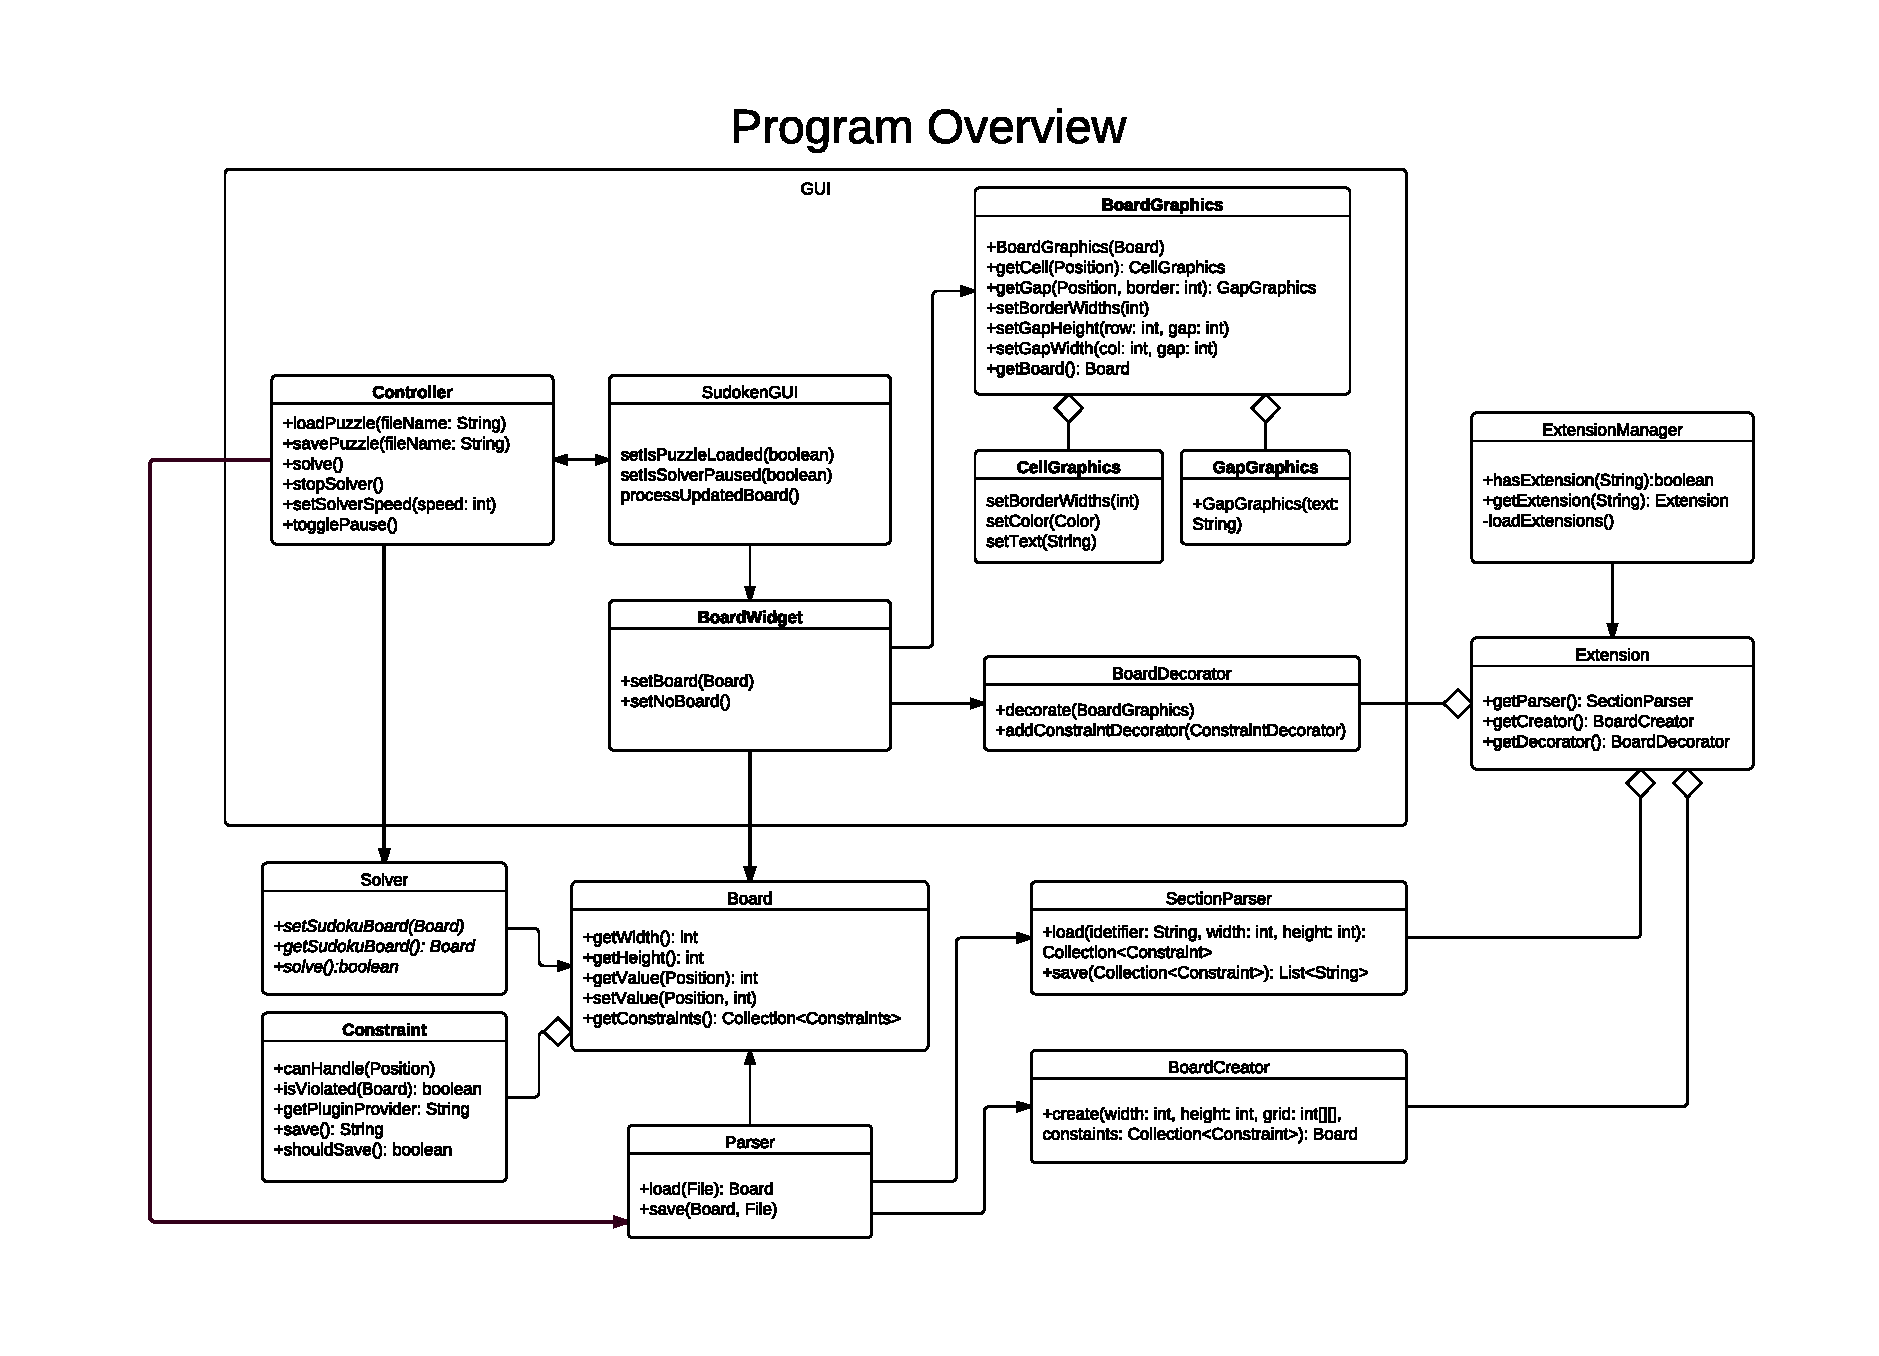
\includegraphics[width=\textwidth]{FrameworkOverview.pdf}
\caption{UML class diagram showing key components of the design}
\end{figure}

\section{Design Patterns}

\subsection{Model-View-Controller}

The \textit{Model-View-Controller} pattern is used to completely separate the presentation layer of the program from the domain logic layer (i.e. separating the \textit{view} from the \textit{model}). These layers should be decoupled to allow them to be independent of one another, as the presentation layer should not need to be aware of the logic layer, and vice versa. This allows the graphical user interface to be changed, or a new interface to be added, without the need for modifying any of the logic layer. It similarly allows changes to the logic layer while requiring changes in the presentation layer.

\begin{table}[h!]
\centering
\begin{tabular}{l l}
\textbf{Role} & \textbf{Binding} \\ \hline
Model         & \texttt{Solver} \\
View          & \texttt{SudokenGUI} \\
Controller    & \texttt{Controller} \\
\end{tabular}
\caption{\textit{Model-View-Controller} pattern.}
\label{table:mvc}
\end{table}

As shown in Table~\ref{table:mvc}, the \textit{model} is implemented as the \texttt{Solver} interface. The \texttt{Solver} contains a \texttt{Board}, which stores all information relating to the puzzle board and its current state. The method \texttt{Solver.solve()} is able to solve the current puzzle.

The \textit{view} is implemented by the \texttt{SudokenGUI} class. This class is responsible for displaying the application on the screen, including drawing the current puzzle board. It has a reference to \texttt{Controller}, the \textit{controller} that mediates communication between the \textit{model} and \textit{view}. Whenever \texttt{SudokenGUI} wants to perform any action to do with the logic of the program, it calls the relevant method of the \texttt{Controller}, e.g., \texttt{loadPuzzle()} when the user wants to load a new puzzle. \texttt{SudokenGUI} does not know anything about how the logic is performed, other than calling these methods on the \texttt{Controller}.

The \texttt{Controller} class has a reference to both the \texttt{SudokenGUI} and \texttt{Solver}, and controls how the \texttt{Solver} and other domain logic should be handled when the user performs actions. The \texttt{Controller} is unaware of how the GUI works or what the user needs to do to fire events, and is similarly unaware of how the \texttt{Solver} solves the \texttt{Board} or what constitutes a \texttt{Board}.

The use of this pattern means that the GUI does not contain any state, and just delegates all actions to the \textit{controller}. The \textit{controller} interacts with the \textit{model} on behalf of the GUI, and interprets any results, changing the GUI accordingly.

This decoupling allows the user interface and the domain model to be developed and tested independently of one another. It facilitates code reuse and extension, as GUIs and models can be interchanged with alternative implementations. It also makes it easier to develop, as the problem is split up and easier to digest by the designers and programmers.

\subsection{Service Locator}

The \textit{Service Locator} pattern is used to allow new puzzle extensions to be hotswapped into the application as it is running. For example, a new \texttt{Extension} packaged into a JAR file can be placed into the plugins directory while the application is running, and it will detect that this new \texttt{Extension} has been added and will load these classes, allowing the user to load and solve puzzles of this type.

The \texttt{ExtensionManager} periodically checks the plugin directory for new JAR files. When these new JAR files are found, they are loaded into the application using \texttt{java.util.ServiceLoader}. The \texttt{Extension Manager} then registers the newly loaded \texttt{Extension}s, placing them in a \texttt{Map} where they are referenced by a string, allowing the program to obtain the appropriate constructors, parsers, and decorators of the extension when needed.

\subsection{Factory Method}

When a puzzle file is loaded into the application, the \texttt{Parser} queries the \texttt{ExtensionManager} to get the \texttt{BoardCreator} of the type of puzzle that is loaded. This \texttt{BoardCreator} is implemented by extensions, such as the \texttt{FutoshikiCreator} for Futoshiki puzzles, and it has a \texttt{create()} method that returns a \texttt{Board}. This is an example of the \textit{factory method} pattern, although the \texttt{Board} class is not extension-specific. Each \textit{ConcreteCreator} instead returns a \texttt{Board} with constraints specific to it, constraints which may or may not be parsed from the puzzle file. The bindings for this pattern in Sudoken are listed in Table~\ref{table:factory}.

\begin{table}[h!]
\centering
\begin{tabular}{l l}
\textbf{Role}   & \textbf{Binding} \\ \hline
Creator         & \texttt{BoardCreator} \\
ConcreteCreator & \texttt{SudokuCreator}, \texttt{FutoshikiCreator}, etc. \\
Product         & \texttt{Board} \\
factoryMethod() & \texttt{create()} \\
\end{tabular}
\caption{\textit{Factory method} pattern.}
\label{table:factory}
\end{table}

The use of this pattern means that the creation of boards and their constraints are delegated to the extensions themselves, and the \texttt{Parser} does not need to know anything about the extension or its constraints, other than the name of the extension (which is specified in the puzzle file). The pattern also allows different extensions to create \texttt{Board}s in their own way, with the functionality of \texttt{create()} being defined in implementations of \texttt{BoardCreator}. Extensions are also able to define and implement their own \texttt{Constraint}s.

\subsection{Strategy}

As a \texttt{Board} is defined by a grid of values and a collection of \texttt{Constraint}s, it is possible to make different implementations of \texttt{Solver}s that will work for any puzzle type. The only requirement is that the entire grid can be filled with values while none of the \texttt{Constraint}s are violated. \texttt{Constraint.isViolated()} is used for this purpose. This allows different strategies to be implemented to solve puzzles (i.e. the \textit{Strategy} pattern). Sudoken's implementations for the roles of this pattern are detailed in Table~\ref{table:strategy}.

\begin{table}[h!]
\centering
\begin{tabular}{l l}
\textbf{Role}        & \textbf{Binding} \\ \hline
Strategy             & \texttt{Solver} \\
ConcreteStrategyA    & \texttt{BacktrackingSolver} \\
ConcreteStrategyB    & \texttt{SmartBacktrackingSolver} \\
AlgorithmInterface() & \texttt{solve()} \\
\end{tabular}
\caption{\textit{Factory method} pattern.}
\label{table:strategy}
\end{table}

This pattern would make it possible so that different \texttt{Solver}s could be loaded and used at runtime. Any implementation of a \texttt{Solver} will be able to solve any puzzle type, but due to their different algorithms, they can take varying amounts of time to solve different types of puzzles---some \texttt{Solver}s will be more suited to solve particular puzzles, but may be less suited for other puzzles.

\subsection{Facade}

Each \texttt{Extension} needs to have a significant amount of control over the display of the board, including features which are not necessarily known by the main application. For example, Futoshiki puzzles will need to display inequality symbols between some cells. However, it is known that the display of each puzzle will follow a general pattern---a grid of cells each containing a value, and that the spaces between cells with often need to be modified for borders, constraint symbols, etc. To allow extensions to have a lot of control of the display of the board while still making it simple for them to implement changes in the board, the \textit{facade} pattern was used.

The \textit{Facade} simplifies this control by offering \texttt{BoardGraphics}, \texttt{CellGraphics}, and \texttt{GapGraphics} classes, each extending \texttt{JPanel}. Together, these classes hide most of the creation and organisation needed to display the board, for example, the creation of the grid layout and display of cell values. Extensions can then customise the board display by calling methods such as \texttt{CellGraphics.setColor()}, which will set the background colour of a particular cell. Most extensions should be able to rely on these access points provided by these classes, but in the event that they need to modify the board in some other way, they can use \texttt{JPanel}'s methods to customise them in any way they want. So, while much of the \texttt{JPanel} functionality can be ignored by extensions, it is still available for their use if they require it.

\subsection{Observer}

The \textit{Observer} pattern is used to notify the GUI that the board has been updated, for example, when a new board has been loaded or a puzzle is being solved. \texttt{SudokenGUI} implements \texttt{BoardChangeListener}, and is added as a listener to the \texttt{Solver} when the application is started. Whenever the board changes and needs to be redrawn, the \texttt{Solver} notifies its listeners (i.e. (\texttt{SudokenGUI}) of the change. \texttt{SudokenGUI} then attempts to redraw the board, based on the current values contained in the cells in the \texttt{Board} and the \texttt{Decorator}s that are applicable. The implemented bindings for the \textit{Observer} pattern are outlined in Table~\ref{table:observer}.

        \begin{table}[h!]
        \centering
        \begin{tabular}{l l}
        \textbf{Role}              & \textbf{Binding} \\ \hline
        Subject                    & \texttt{Solver} \\
        Subject.registerObserver() & \texttt{Solver.addListener()} \\
        Subject.notifyObservers()  & \texttt{Solver.notifyListeners()} \\
        Observer                   & \texttt{BoardChangeListener} \\
        Observer.notify()          & \texttt{BoardChangeListener.processUpdatedBoard()} \\
        ConcreteObserver           & \texttt{SudokenGUI} \\
        \end{tabular}
        \caption{\textit{Observer} pattern.}
        \label{table:observer}
        \end{table}

The \textit{Observer} pattern here makes it possible for \texttt{SudokenGUI} to update whenever \texttt{Solver} changes the board state, with these classes decoupled from each other. This decoupling minimises the amount of modifications needed if related parts of the program are refactored in the future. Another advantage is that new functionality which depends on knowing when the board changes can do so by simply becoming a listener of \texttt{Solver}. In other words, \texttt{Solver} and the puzzle board are open for extension, but not for modification.

\end{document}
